\documentclass[11pt,a4paper]{article}
\usepackage[margin=1in]{geometry}
\usepackage[T1]{fontenc}
\usepackage[utf8]{inputenc}
\usepackage{lmodern}
\usepackage{hyperref}
\usepackage{enumitem}
\usepackage{xurl}
\usepackage{tikz}
\usepackage{float}
\usetikzlibrary{arrows.meta, positioning, shapes.geometric}
\hypersetup{colorlinks=true,linkcolor=blue,urlcolor=blue}
\newcommand{\codepath}[1]{\path{#1}}
\tikzset{box/.style={rectangle,draw,rounded corners,align=center,inner sep=3pt,minimum width=36mm},decision/.style={diamond,draw,aspect=2.1,align=center,inner sep=2pt},line/.style={-Latex}}

\title{Phase-2 Deliverable: CI Integration}
\author{SIT Engine Architecture}
\date{\today}

\begin{document}
\maketitle

\section{Technical Description}
CI integration provides deterministic merge gates for replay and conformance checks. It ensures changes to adapters, workloads, and orchestration do not silently regress SIT behavior.

\section{Implementation Fulfillment}
Current repository state:
\begin{itemize}[leftmargin=*]
  \item Phase-1 workflow exists: \codepath{.github/workflows/phase1-ci.yml},
  \item reusable Phase-2 commands already exist:
  \begin{itemize}
    \item \codepath{Phase-2/tests/check_adapter_fixtures.py},
    \item \codepath{Phase-2/tests/check_determinism.py},
    \item \codepath{Phase-2/run_cross_target_suite.py},
    \item \codepath{Phase-2/tests/run_golden_suite.py}.
  \end{itemize}
\end{itemize}
Known gap: dedicated \codepath{.github/workflows/phase2-ci.yml} is not yet present.

\section{Design \& Architecture}
Recommended CI topology:
\begin{itemize}[leftmargin=*]
  \item fast PR gate (fixtures + qemu determinism + smoke subset),
  \item optional/nightly extended lane (Spike/gem5 full golden matrix),
  \item fail-fast policy with artifact retention for triage.
\end{itemize}
CI should orchestrate checks only; validation logic remains in test scripts.

\subsection*{Function Flowchart}
\begin{figure}[H]
\centering
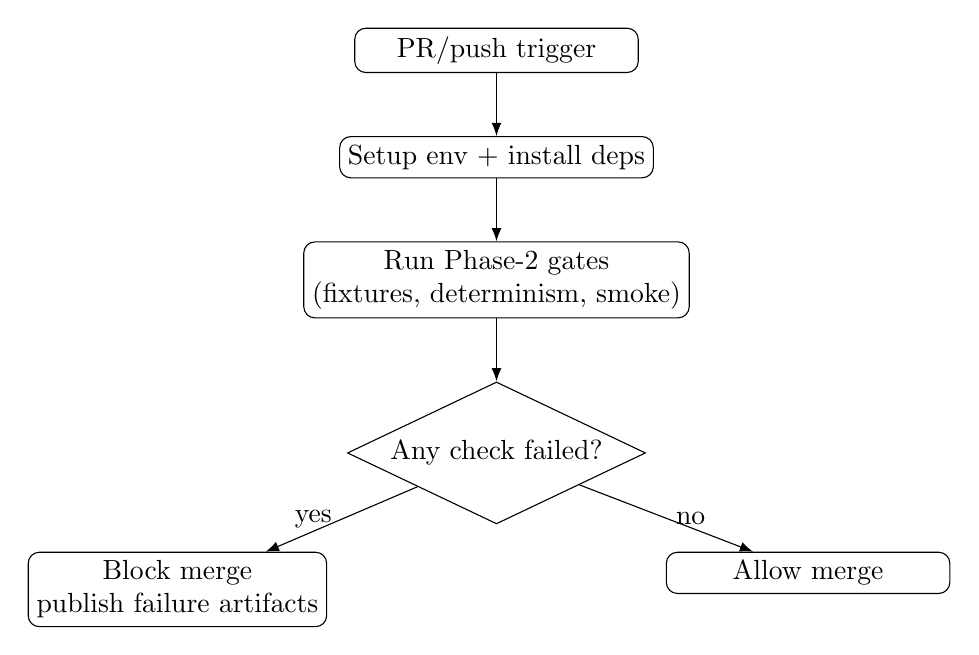
\begin{tikzpicture}[node distance=8mm and 12mm]
\node[box] (a) {PR/push trigger};
\node[box, below=of a] (b) {Setup env + install deps};
\node[box, below=of b] (c) {Run Phase-2 gates\\(fixtures, determinism, smoke)};
\node[decision, below=of c] (d) {Any check failed?};
\node[box, below left=of d] (e1) {Block merge\\publish failure artifacts};
\node[box, below right=of d] (e2) {Allow merge};
\draw[line] (a) -- (b);
\draw[line] (b) -- (c);
\draw[line] (c) -- (d);
\draw[line] (d) -- node[left]{yes} (e1);
\draw[line] (d) -- node[right]{no} (e2);
\end{tikzpicture}
\caption{Phase-2 CI Integration Flow}
\end{figure}

\end{document}
